% Created 2024-04-28 Sun 15:18
% Intended LaTeX compiler: pdflatex
\documentclass[11pt]{article}
\usepackage[utf8]{inputenc}
\usepackage[T1]{fontenc}
\usepackage[margin=0.5in]{geometry}
\usepackage{graphicx}
\usepackage{longtable}
\usepackage{wrapfig}
\usepackage{rotating}
\usepackage[normalem]{ulem}
\usepackage{amsmath}
\usepackage{amssymb}
\usepackage{capt-of}
\author{Martin Chaperot: 20205638 \\ Hamza Ali Ousalah: 20249230}
\date{}
\title{Devoir 4 Rapport}

\begin{document}

\maketitle

\section{Q1}
\subsection{a}
\begin{center}
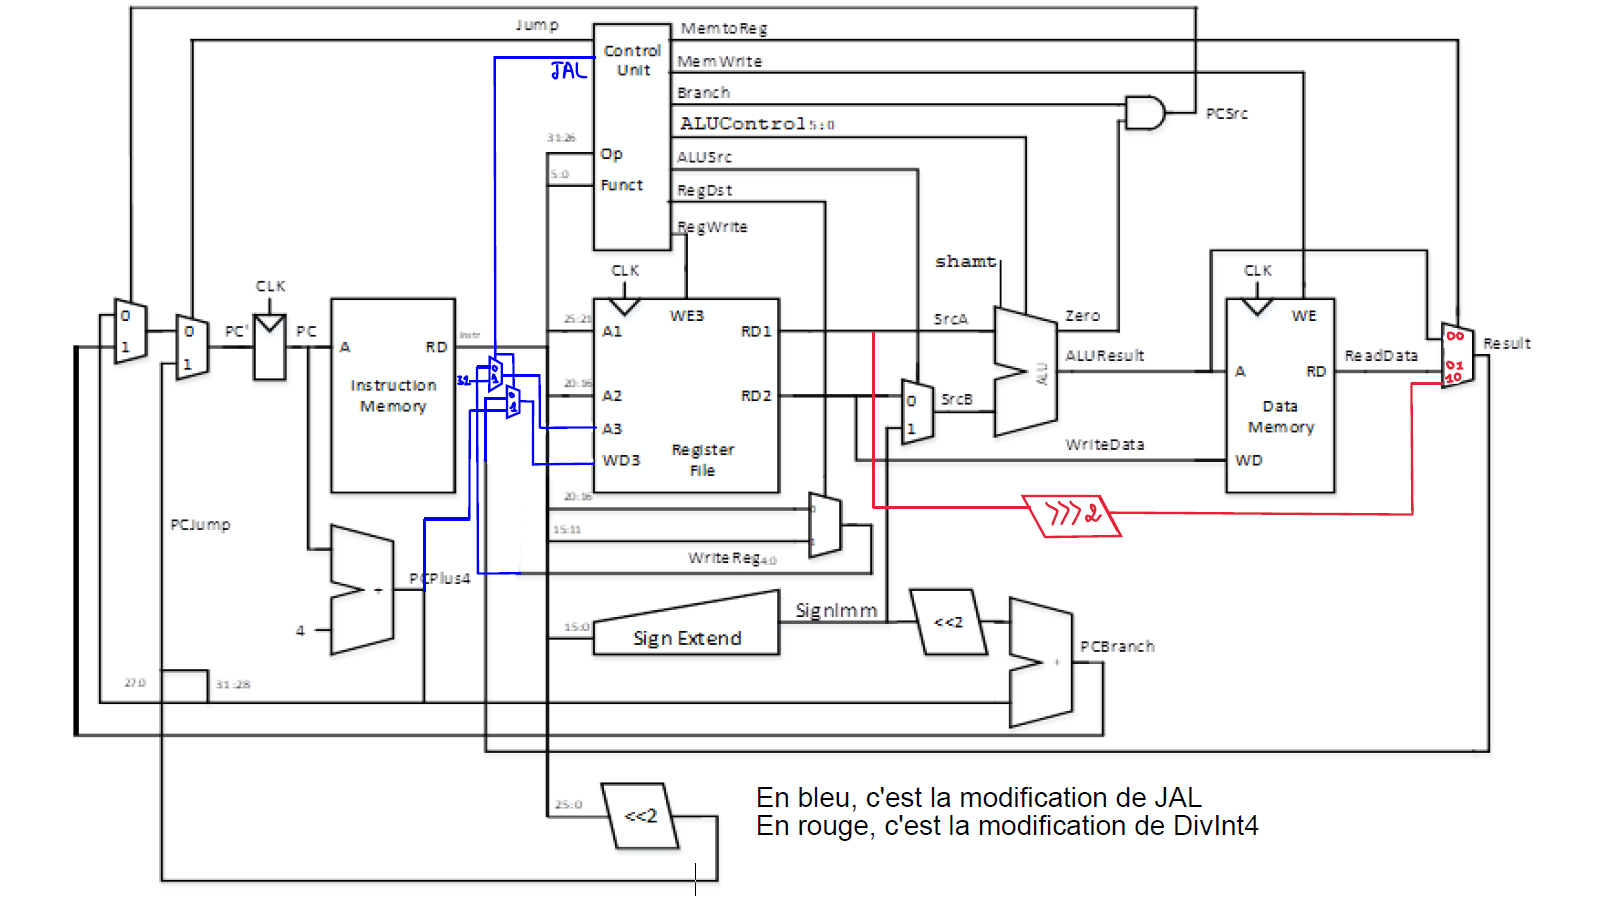
\includegraphics[width=.9\linewidth]{./Question_1_a.png}
\end{center}
\subsection{b}
\begin{center}
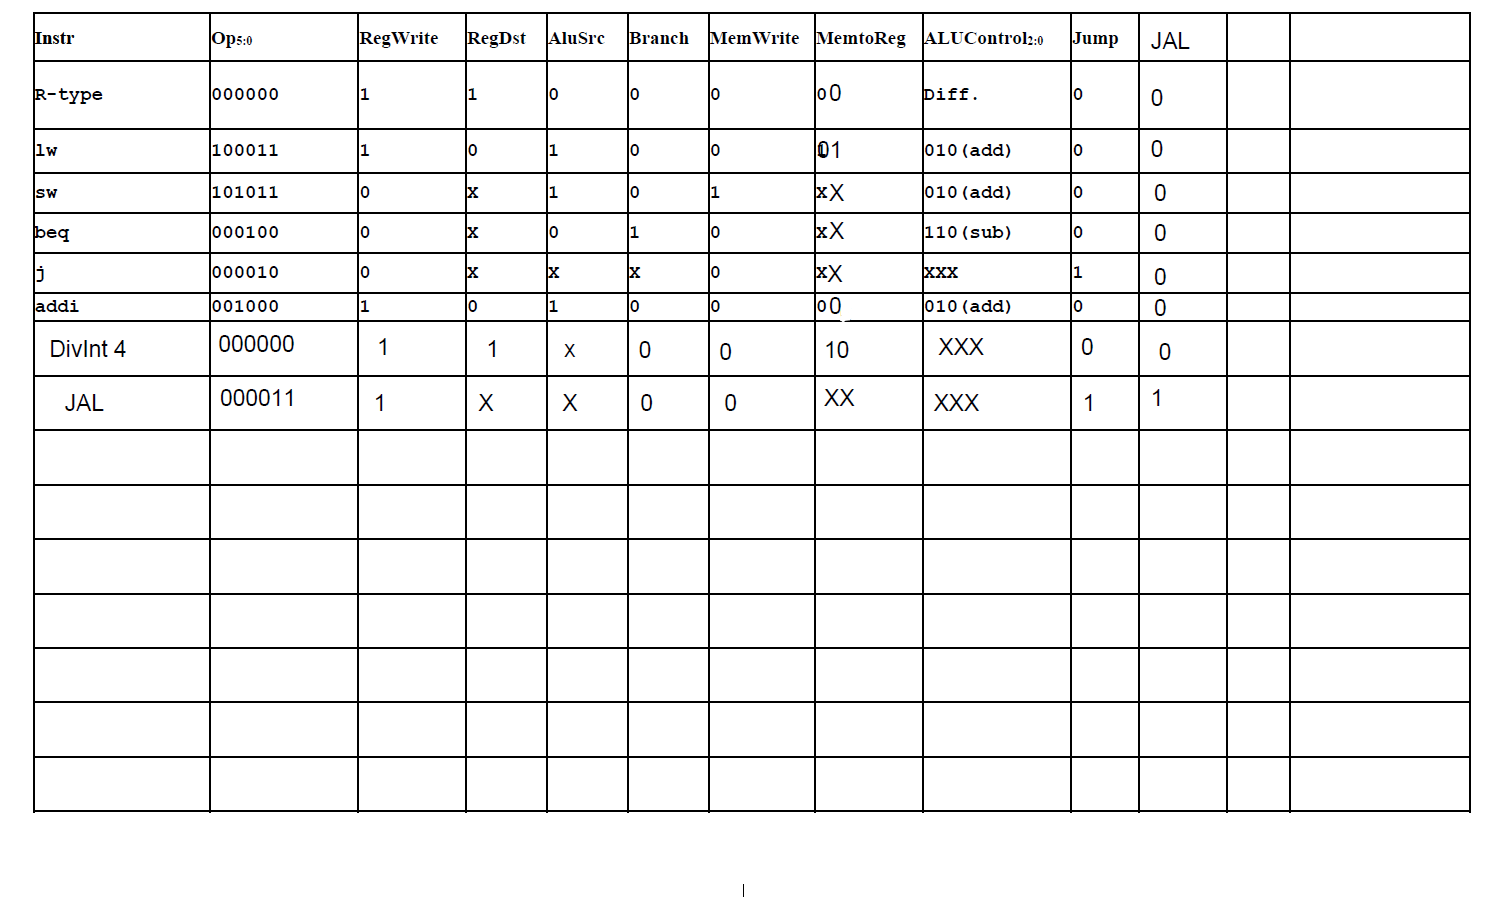
\includegraphics[width=.9\linewidth]{./Question_1_b.png}
\end{center}
\section{Q2}
imem.vhd (Programme de test avec le code assembleur et le code machine)
\begin{verbatim}
library IEEE;
use IEEE.STD_LOGIC_1164.all; 
use STD.TEXTIO.all;
use IEEE.STD_LOGIC_UNSIGNED.all; use IEEE.STD_LOGIC_ARITH.all;

entity imem is -- instruction memory, TP4 
        port (	a : 	in STD_LOGIC_VECTOR (5 downto 0);
                           rd:   out STD_LOGIC_VECTOR (31 downto 0));
end;

architecture behave of imem is
begin
        process(a)
                type ramtype is array (63 downto 0) of STD_LOGIC_VECTOR(31 downto 0);
                variable mem: ramtype;
        begin
        -- initialize memory 
        mem(0)  := X"20020005";	--addi $v0, $0, 5	   # $v0(2) = 5
        mem(1)  := X"2003000c";	--addi $v1, $0, 12	   # $v1(3) = 12
        mem(2)  := X"2067fff7";	--addi $a3, $v1,-9 	# $a3(7) = $v1(3)(12) - 9 = 3
        mem(3)  := X"00e22025";	--or   $a0, $a3, $v0	# $a0(4) = $a3(7) or $v0(2) = 3 or 5 = 7
        mem(4)  := X"00642824";	--and  $a1, $v1, $a0	# $a1(5) = $v1(3) and $a0(4)= 12 and 7 = 4
        mem(5)  := X"00a42820";	--add  $a1, $a1, $a0	# $a1(5) = $a1(5) + $a0(4) = 4 + 7 = 11
        mem(6)  := X"10a7000a";	--beq  $a1, $a3, end	# $a1(5)==$a3(7)? end: PC=PC+4; 11==3 ? PC=PC+4
        mem(7)  := X"0064202a";	--slt  $a0, $v1, $a0	# $v1(3)<$a0(4) ? $a0 = 1 : $a0 = 0; 
        mem(8)  := X"10800001";	--beq  $a0, $0, ar1	# $a0(4)==0?ar1:PC = PC+4; 0==0 goto ar1 
        mem(9)  := X"20050000";	--addi $a1, $0, 0		# 
        mem(10) := X"00e2202a";	--ar1: slt $a0, $a3, $v0	# $a3(7)<$v0(2)?$a0(4)=1:$a0=0; 3<5,$a0=1
        mem(11) := X"00853820";	--add 	$a3, $a0, $a1	# $a3(7)=$a0(4)+$a1(5); 1+11=12
        mem(12) := X"00e23822";	--sub 	$a3, $a3, $v0	# $a3(7)=$a3(7)-$v0(2); 12-5=7
        mem(13) := X"ac670044";	--sw 	$a3, 68($v1)	# $a3(7)->M[68+$v1(3)]; 7->M[68+12=80] #test 1
        mem(14) := X"8c020050";	--lw 	$v0, 80($0)		# $v0(2) = M[80+0]; $v0 = 7
        mem(15) := X"08000011";	--j 	end			   # goto end
        mem(16) := X"20020001";	--addi $v0, $0, 1
        mem(17) := X"ac02003C";	--end: sw $v0, 60($0) 	# $v0(2) write M[60]; M[60]=7; #test 2
        mem(18) := X"0022180A"; --divInt4 $v1, $v0 # ($v1 = $v0 / 4)
        mem(19) := X"ac010028"; --sw $v1, 40($0) # divInt4 test
        mem(20) := X"0c000015"; --jal jalTest
        mem(21) := X"AC3E0014"; --sw $ra, 30($0) # jal test
        for ii in 22 to 63 loop
            mem(ii) := X"00000000";
        end loop;  -- ii
        -- read memory
        rd <= mem(CONV_INTEGER(a));
end process;
end;
\end{verbatim}
\section{Q3}
\subsection{a}
\begin{center}
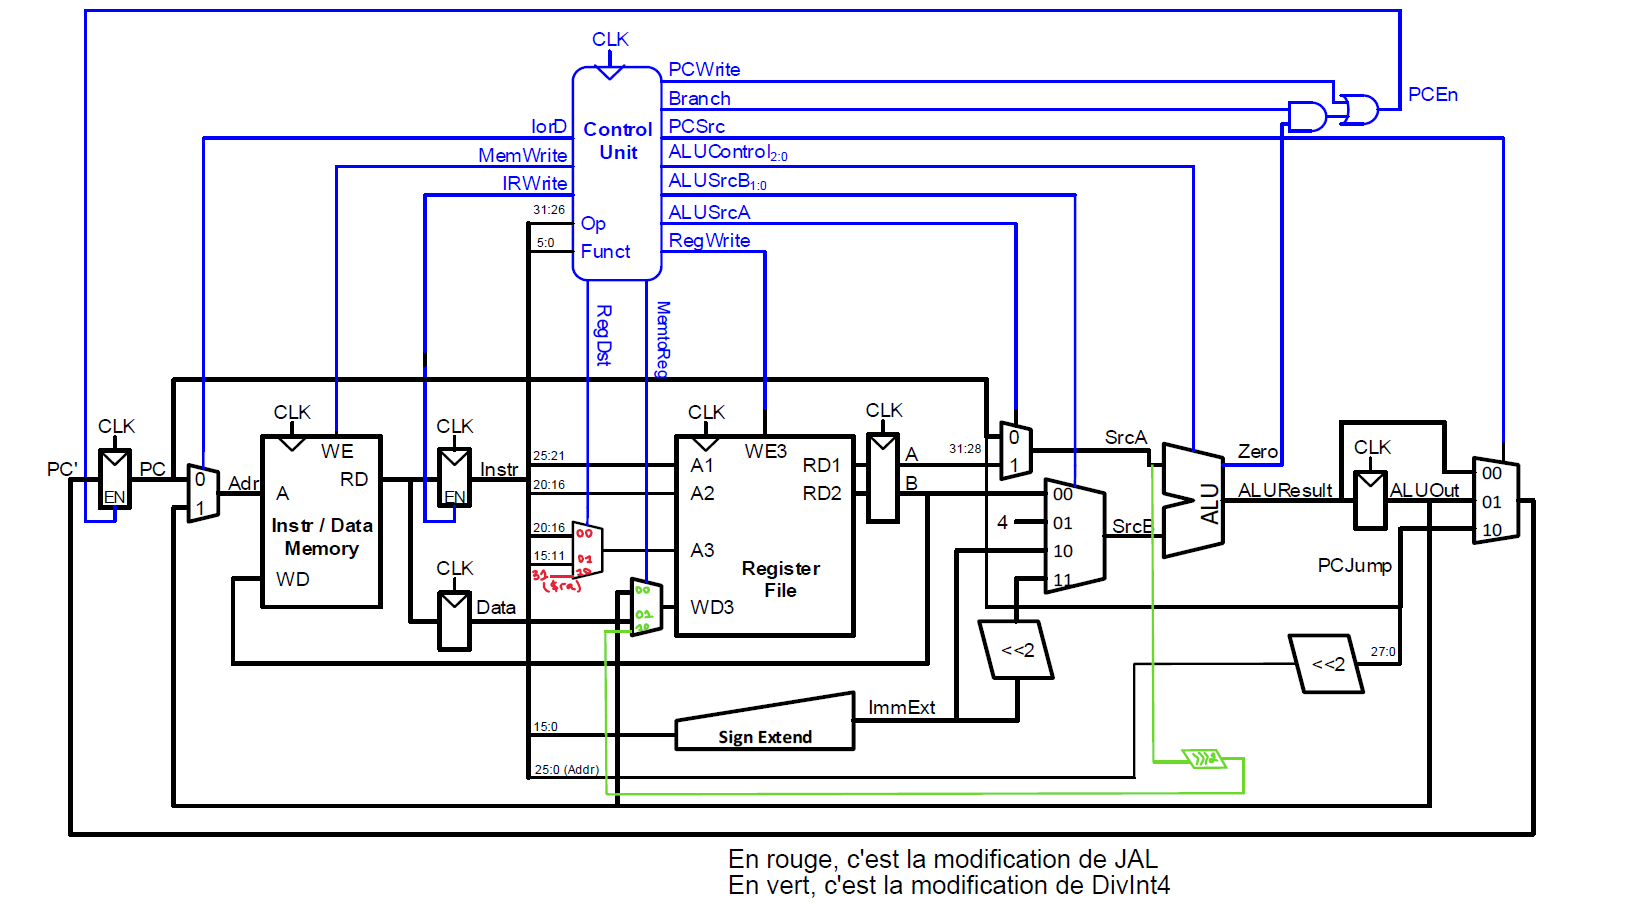
\includegraphics[width=.9\linewidth]{./Question_3_a.png}
\end{center}
\subsection{b}
\begin{center}
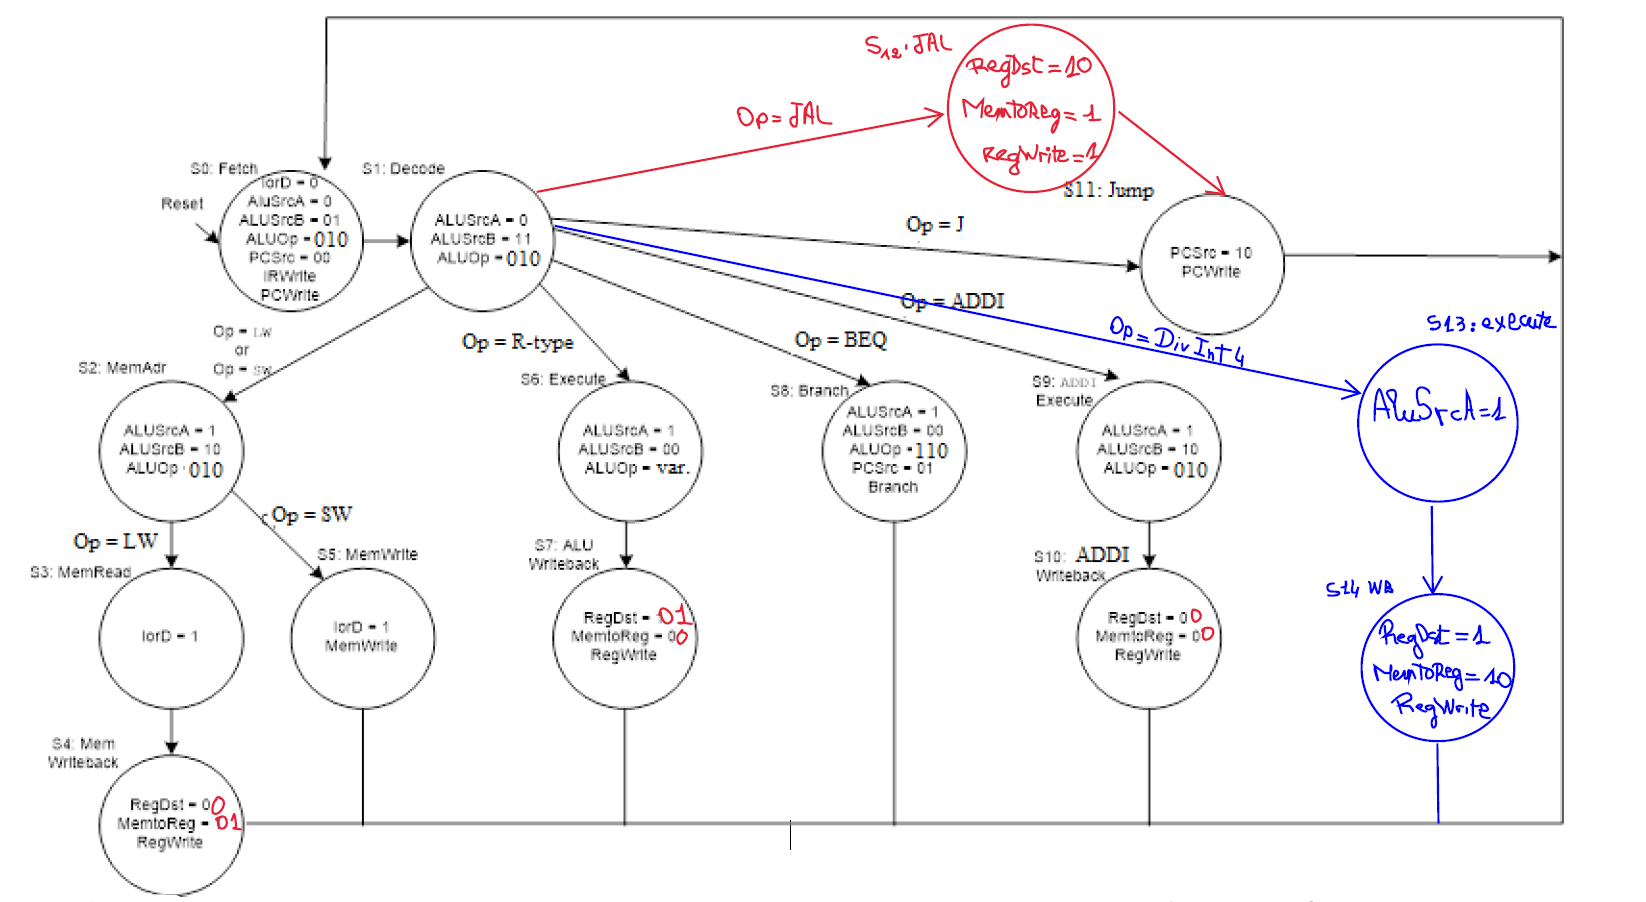
\includegraphics[width=.9\linewidth]{./Question_3_b.png}
\end{center}
\end{document}
